\documentclass[aspectratio=169]{beamer}
\usetheme{Madrid}
\usefonttheme{structurebold}
\usefonttheme[onlymath]{serif}
%\usepackage[utf8]{vietnam}
\definecolor{BKTemplate}{rgb}{0.11765, 0.30588, 0.47451}
\usecolortheme[named=BKTemplate]{structure}
\setbeamercolor{title}{fg=BKTemplate,bg=} 
\setbeamertemplate{caption}[numbered]

\usepackage{bookmark}
\usepackage{lmodern}
\usepackage{graphicx}
\usepackage{amsmath}
\usepackage{tcolorbox}
\usepackage[export]{adjustbox}
\usepackage{caption}
\usepackage{array}
\usepackage[utf8]{inputenc}
\usepackage[T1]{fontenc}    % use 8-bit T1 fonts
\usepackage{url}            % simple URL typesetting
\usepackage{booktabs}       % professional-quality tables
\usepackage{amsfonts}       % blackboard math symbols
\usepackage{nicefrac}       % compact symbols for 1/2, etc.
\usepackage{microtype}      % microtypography
\microtypesetup{expansion=false}
\usepackage{mathtools}
\usepackage{multicol}
\usepackage{comment}
\usepackage{forest}
\usepackage[linesnumbered, ruled]{algorithm2e}
\usepackage{algorithmic}
\usepackage{xcolor}
\usepackage{colortbl}
\usepackage{graphicx}
\usepackage{diagbox}
\usepackage{tikz}
\usepackage{subcaption}
% \captionsetup[subfigure]{labelsep=space}
\usepackage{amsmath}
\usepackage{dsfont}
\usepackage{stmaryrd}
\usepackage[style=authortitle,backend=biber]{biblatex}
\addbibresource{thesiscite.bib}
\renewcommand{\footnotesize}{\tiny}
\newcommand{\mathbi}[1]{\boldsymbol{#1}}
\newtheorem{proposition}{Proposition}

%------------------------------------------------------------
%This block of code defines the information to appear in the
%Title page

\title[SEMINAR] %optional
{\vspace*{1cm}\\\textbf{SEMINAR}\\\textbf{Vision-Language Models Survey}}

\subtitle{}

% \author % (optional)
% {Supervisor:  Associate Professor Dr. Le Hong Trang\\
% Student: Cao Thanh Bang - Phan Dinh Cuong}

\institute[HCMUT] % (optional)
{
  Faculty of Computer Science and Engineering\\
  Ho Chi Minh City University of Technology\\
  Vietnam National University Ho Chi Minh City
}

\date[July 2025] 

%End of title page configuration block
%------------------------------------------------------------



%------------------------------------------------------------
%The next block of commands puts the table of contents at the 
%beginning of each section and highlights the current section:

%------------------------------------------------------------


\AtBeginSection[]
{
  \begin{frame}
    \frametitle{Table of Contents}
    \tableofcontents[currentsection]
  \end{frame}
}
\begin{document}

% The next statement creates the title page.
\setbeamertemplate{background canvas}{
	\includegraphics[width=\paperwidth,height=\paperheight]{images/FrontBackground.pdf}
}
\begin{frame}[plain]
\titlepage
\end{frame}


% Set background for all pages
\setbeamertemplate{background canvas}{
	\includegraphics[width=\paperwidth,height=\paperheight]{images/Background.pdf}
}

%---------------------------------------------------------
%This block of code is for the table of contents after
%the title page
\begin{frame}
\frametitle{Table of Contents}
\tableofcontents
\end{frame}

\section{Background}
\begin{frame}{Background}
With the advent of deep learning, visual recognition research has achieved great success by leveraging end-to-end trainable deep neural networks (DNNs).
\vspace{1em}
However, the shift from traditional machine learning to deep learning comes with two new grand challenges: \begin{itemize}
        \item The slow convergence of DNN training under the classical setup of Deep Learning from scratch
        \item The laborious collection of large-scale, task specific, and crowd-labelled data in DNN training.
    \end{itemize}
\end{frame}
\begin{frame}{Background}
\begin{itemize}
    \item Recently, a new learning paradigm Pre-training, Finetuning and Prediction has demonstrated great effectiveness in a wide range of visual recognition tasks.
    \vspace{1em}
    \item Inspired by the advances in natural language processing, a new deep learning paradigm named Vision-Language Model Pre-training and Zero-shot Prediction has appeared.
\end{itemize}

\begin{figure}
    \centering
    \includegraphics[width=0.6\linewidth]{images/increasing_published_papers.png}
    \caption{ Number of publications on visual recognition VLMs
 (from Google Scholar)}
\end{figure}

\end{frame}



\section{Introduction}
\begin{frame}{Introduction}
\begin{block}{Definition}
VLMs learn to map the relationships between text data and visual data such as images or videos, allowing these models to generate text from visual input or understand natural language commands in the context of visual information\footnotemark.
\end{block}

\begin{figure}
    \centering
    \includegraphics[width=0.6\linewidth]{images/vision_language_model_outline.png}
    \caption{Visualization of a Vision-Language Model}
\end{figure}

\footnotetext{\url{https://www.ibm.com/think/topics/vision-language-models}}
\end{frame}

\begin{frame}{Introduction}
\begin{block}{Core Capabilities}
\begin{itemize}
    \item Unlike traditional computer vision models, VLMs are not bound by a fixed set of classes or a specific task such as classification or detection.
    \item Retrained on a vast corpus of text and image / video caption pairs, VLMs can be trained in natural language and used to handle many classic vision tasks plus new AI-powered generative tasks such as summarization and visual question answering.
\end{itemize}
\end{block}
\begin{figure}
    \centering
    \includegraphics[width=0.6\linewidth]{images/vision_language_model_outline2.png}
    \caption{Illustrations of Visual Question Answering}
\end{figure}
\end{frame}

\begin{frame}{Introduction}
\begin{figure}
    \centering
    \includegraphics[width=0.6\linewidth]{images/intro_image.png}
    \caption{Three DNN training paradigms in visual recognition.}
\end{figure}
\end{frame}


\begin{frame}{Introduction}
\centering
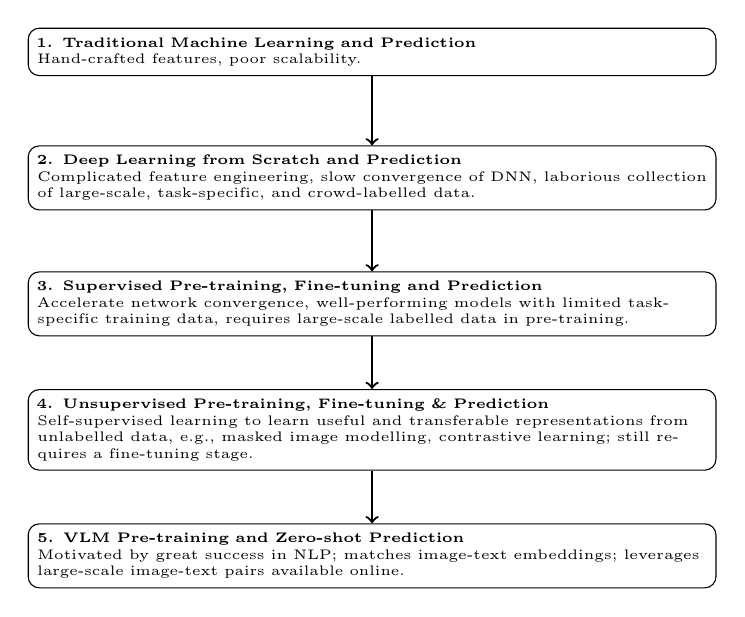
\begin{tikzpicture}[
  node distance=1.6cm,
  every node/.style={rectangle, draw=black, rounded corners, align=left, text width=8.5cm, font=\footnotesize, fill=white},
  line/.style={->, thick, draw=black}
]

\node (block1) {\textbf{1. Traditional Machine Learning and Prediction}\\
Hand-crafted features, poor scalability.};

\node (block2) [below of=block1] {\textbf{2. Deep Learning from Scratch and Prediction}\\
Complicated feature engineering, slow convergence of DNN, laborious collection of large-scale, task-specific, and crowd-labelled data.};

\node (block3) [below of=block2] {\textbf{3. Supervised Pre-training, Fine-tuning and Prediction}\\
Accelerate network convergence, well-performing models with limited task-specific training data, requires large-scale labelled data in pre-training.};

\node (block4) [below of=block3] {\textbf{4. Unsupervised Pre-training, Fine-tuning \& Prediction}\\
Self-supervised learning to learn useful and transferable representations from unlabelled data, e.g., masked image modelling, contrastive learning; still requires a fine-tuning stage.};

\node (block5) [below of=block4] {\textbf{5. VLM Pre-training and Zero-shot Prediction}\\
Motivated by great success in NLP; matches image-text embeddings; leverages large-scale image-text pairs available online.};

% Arrows
\draw [line] (block1) -- (block2);
\draw [line] (block2) -- (block3);
\draw [line] (block3) -- (block4);
\draw [line] (block4) -- (block5);

\end{tikzpicture}
\end{frame}


\section{Vision-Language Tasks and Variants}
\section{Vision-language tasks and variants}

\begin{frame}{Vision-language tasks and variants}
\begin{block}

Early VLMs focus on image-level visual recognition tasks, whereas recent VLMs are more general-purpose, which can also work for dense prediction tasks that are complex and require localization related knowledge.
\end{block}
\end{frame}

\begin{frame}{Table 1: Core Vision Tasks}
\begin{table}[h!]
\centering
\resizebox{\textwidth}{!}{%
\begin{tabular}{|l|l|l|}
\hline
\textbf{Task Type}             & \textbf{Description}                                                & \textbf{Strong VLM Models}                       \\ \hline
\textbf{Image Classification}  & Predicts a label for the whole image (e.g., bear, dog, car...)     & \textbf{CLIP}, \textbf{BLIP}, \textbf{ALIGN}, \textbf{Florence} \\ \hline
\textbf{Object Detection}      & Detects multiple objects with bounding boxes                        & \textbf{Grounding DINO}, \textbf{OWL-ViT}, \textbf{GLIP}         \\ \hline
\textbf{Semantic Segmentation} & Labels each pixel by class (not separating instances)               & \textbf{CLIPSeg}, \textbf{LSeg}                                 \\ \hline
\textbf{Instance Segmentation} & Labels and distinguishes each object instance individually          & \textbf{SAM}, \textbf{SEEM}, \textbf{GRIT}                      \\ \hline
\end{tabular}%
}
\end{table}
\end{frame}

\begin{frame}{Table 2: Advanced Multimodal Tasks}
\begin{table}[H]
\centering
\resizebox{\textwidth}{!}{%
\begin{tabular}{|l|l|l|}
\hline
\textbf{Task Type} & \textbf{Description} & \textbf{Strong VLM Models} \\
\hline
Image Captioning & Generates a text description for the image & \textbf{BLIP}, \textbf{BLIP-2}, \textbf{GIT}, \textbf{MiniGPT-4} \\
\hline
Visual Question Answering (VQA) & Answers questions based on the image content & \textbf{BLIP-2}, \textbf{Flamingo}, \textbf{MiniGPT-4}, \textbf{LLaVA} \\
\hline
Visual Grounding & Locates regions in the image based on a textual description & \textbf{Grounding DINO}, \textbf{OWL-ViT}, \textbf{GLIP} \\
\hline
Text-to-Image Retrieval & Finds matching images from a text query (or vice versa) & \textbf{CLIP}, \textbf{ALIGN}, \textbf{Florence} \\
\hline
Multimodal Reasoning & Performs reasoning using both image and language modalities & \textbf{GPT-4V}, \textbf{Kosmos-2}, \textbf{MiniGPT-4}, \textbf{LLaVA} \\
\hline
\end{tabular}%
}
\end{table}
\end{frame}


\begin{frame}{VLMs on vision tasks}
\begin{figure}
    \centering
    \includegraphics[width=0.6\linewidth]{images/benchmarking_on_classif_tasks_clip.png}
    \caption{ ResNet-101 fine-tuned on ImageNet vs. zero-shot CLIP}
\end{figure}
\end{frame}

\begin{frame}{VLMs on vision tasks}
\begin{figure}
    \centering
    \includegraphics[width=0.6\linewidth]{images/CLIPSeg.png}
    \caption{Basic processing systems apply CLIPSeg for Object Segmentation tasks}
\end{figure}
\end{frame}

\begin{frame}{VLMs on vision tasks}
\begin{figure}
    \centering
    \includegraphics[width=0.6\linewidth]{images/Screenshot 2025-07-20 101518.png}
    \caption{CLIP in object detection and localization}
\end{figure}
\end{frame}

\section{Current Approaches to VLM}
% Frame 6 - VLM Pre-training Frameworks
\begin{frame}{VLM Pre-training Frameworks}
\textbf{Three curent approached frameworks:}
\begin{itemize}
    \item Two-Tower VLM
    \item Two-Leg VLM
    \item One-Tower VLM
\end{itemize}

\begin{figure}
    \centering
    \includegraphics[width=0.75\linewidth]{images/VLM_Frameworks.png}
    \caption{three current architectures of VLM}
\end{figure}
\end{frame}

\begin{frame}{CNN-based Architectures for Image Features}

\textbf{CNN-based Architectures:}
\begin{itemize}
    \item Different ConvNets such as VGG, ResNet, and EfficientNet have been widely used for learning image features.
    \item These models rely on convolutional layers to capture spatial hierarchies in images.
\end{itemize}

\vspace{0.4cm}

\begin{figure}
    \centering
    \includegraphics[width=0.4\linewidth]{images/CONvNet.png}
    \caption{Convolutional architecture}
\end{figure}

\end{frame}

\begin{frame}{Transformer-based Architectures for Image Features}

\textbf{Vision Transformer (ViT):}
\begin{itemize}
    \item ViT applies Transformer blocks to image patches instead of word tokens.
    \item Each block includes multi-head self-attention and a feed-forward network.
    \item ViT has shown competitive or superior performance compared to CNNs on many visual tasks.
\end{itemize}

\vspace{0.4cm}

\begin{figure}
    \centering
    \includegraphics[width=0.35\linewidth]{images/VT_image.png}
    \caption{Vision transformer architecture}
\end{figure}

\end{frame}



% Frame 2 - Network Architectures (Text)
\begin{frame}{Learning Language Features}
\textbf{Transformer-based Architectures for Language:}
\begin{itemize}
    \item Transformer and its variants are widely used to learn text representations.
\end{itemize}
\begin{figure}
    \centering
    \includegraphics[width=0.3\linewidth]{images/VT_language.png}
    \caption{Vision transformer architecture}
\end{figure}
\end{frame}

\begin{frame}{VLM Pre-training Objectives }
\textbf{VLM Pre-training Objectives}
As the core of VLM, various vision language pre-training objectives have been designed to learn a rich vision-language correlation. 

\vspace{1em}

\textbf{Three types of contrastive learning:}
\begin{itemize}
    \item Contrastive objectives
    \item Generative objectives
    \item Alignment objectives
\end{itemize}
\end{frame}



% Frame 3 - VLM Pre-training Objectives (1)
\begin{frame}{Contrastive Objectives }
\textbf{Contrastive Objectives:}
Learn discriminative representations by pulling paired samples close and pushing others away.

\vspace{1em}

\textbf{Three types of contrastive learning:}
\begin{itemize}
    \item Image Contrastive Learning
    \item Image-Text Contrastive Learning
    \item Image-Text-Label Contrastive Learning
\end{itemize}
\end{frame}

\begin{frame}{Image Contrastive Learning}
\begin{tcolorbox}[colback=blue!5!white, colframe=blue!75!black]
    Given a batch of $B$ images, image contrastive learning (e.g., InfoNCE) aims to bring positive pairs $(z_i^I, z_i^{I+})$ close and push negative keys $z_j^I, j \neq i$ away.
\end{tcolorbox}

\vspace{0.5em}

\begin{block}{Loss Formulation}
\footnotesize
\[
\mathcal{L}_{I}^{\text{InfoNCE}} = -\frac{1}{B} \sum_{i=1}^{B} \log \frac{\exp(z_i^I \cdot z_{i+}^I / \tau)}{\sum_{j=1, j \neq i}^{B+1} \exp(z_i^I \cdot z_j^I / \tau)}
\]
\end{block}

\vspace{0.5em}

\end{frame}



\begin{frame}{Image-text Contrastive Learnings}
\begin{minipage}[t]{0.5\textwidth}
    \includegraphics[width=\linewidth,valign=t]{images/image-text-constrastive-learning.png}
\end{minipage}
\hfill
\begin{minipage}[t]{0.48\textwidth}
    \begin{tcolorbox}[colback=blue!5!white, colframe=blue!75!black]
        pulling the embeddings of paired images and texts close while pushing others 
    \end{tcolorbox}
    
    \vspace{0.5em}
    
    \begin{block}{Loss Formulation}
    \footnotesize
    \[
    \mathcal{L}_{I \rightarrow T} = -\frac{1}{B} \sum_{i=1}^{B} \log \frac{\exp \left( z_i^I \cdot z_i^T / \tau \right)}{\sum_{j=1}^{B} \exp \left( z_i^I \cdot z_j^T / \tau \right)}
    \]
    \[
    \mathcal{L}_{T \rightarrow I} = -\frac{1}{B} \sum_{i=1}^{B} \log \frac{\exp \left( z_i^T \cdot z_i^I / \tau \right)}{\sum_{j=1}^{B} \exp \left( z_i^T \cdot z_j^I / \tau \right)}
    \]
    \end{block}
\end{minipage}
\end{frame}

\begin{frame}{Image-Text-Label Contrastive Learning}
\begin{minipage}[t]{0.5\textwidth}
    \includegraphics[width=\linewidth,valign=t]{images/img-text-label-constrastive.png}
\end{minipage}
\hfill
\begin{minipage}[t]{0.48\textwidth}
    \begin{tcolorbox}[colback=blue!5!white, colframe=blue!75!black]
        Introduces supervised contrastive learning into image-text contrastive learning by grouping samples with the same label as positives.
    \end{tcolorbox}

    \vspace{0.5em}
    
    \begin{block}{Loss Formulation}
    \footnotesize
    \[
    \mathcal{L}_{I \rightarrow T}^{\text{ITL}} = -\sum_{i=1}^{B} \frac{1}{|\mathcal{P}(i)|} \sum_{k \in \mathcal{P}(i)} \log \frac{\exp(z_i^I \cdot z_k^T / \tau)}{\sum_{j=1}^{B} \exp(z_i^I \cdot z_j^T / \tau)}
    \]
    \[
    \mathcal{L}_{T \rightarrow I}^{\text{ITL}} = -\sum_{i=1}^{B} \frac{1}{|\mathcal{P}(i)|} \sum_{k \in \mathcal{P}(i)} \log \frac{\exp(z_i^T \cdot z_k^I / \tau)}{\sum_{j=1}^{B} \exp(z_i^T \cdot z_j^I / \tau)}
    \]
    \end{block}
\end{minipage}
\end{frame}



\begin{frame}{Masked Image Modeling - Generative}
\begin{minipage}[t]{0.5\textwidth}
    \includegraphics[width=\linewidth,valign=t]{images/masked-image-modelling.png}
\end{minipage}
\hfill
\begin{minipage}[t]{0.48\textwidth}
    \begin{tcolorbox}[colback=blue!5!white, colframe=blue!75!black]
        Randomly masks a subset of image patches and trains the model to reconstruct them from the unmasked patches.
    \end{tcolorbox}

    \vspace{0.5em}

    \begin{block}{Loss Formulation}
    \footnotesize
    \[
    \mathcal{L}_{\text{MIM}} = -\frac{1}{B} \sum_{i=1}^{B} \log f_\theta(x_i^I \mid \hat{x}_i^I)
    \]
    \end{block}
    \footnotesize{where $x_i^I$ is the masked patch set and $\hat{x}_i^I$ is the unmasked patch set of image $x_i^I$.}
\end{minipage}
\end{frame}

\begin{frame}{Masked Language Modeling - Generative}
\begin{minipage}[t]{0.5\textwidth}
    \includegraphics[width=\linewidth,valign=t]{images/mask-language-modelling.png}
\end{minipage}
\hfill
\begin{minipage}[t]{0.48\textwidth}
    \begin{tcolorbox}[colback=blue!5!white, colframe=blue!75!black]
        Randomly masks a subset of text tokens and reconstructs them based on the unmasked tokens.
    \end{tcolorbox}

    \vspace{0.5em}

    \begin{block}{Loss Formulation}
    \footnotesize
    \[
    \mathcal{L}_{\text{MLM}} = -\frac{1}{B} \sum_{i=1}^{B} \log f_\phi(x_i^T \mid \hat{x}_i^T)
    \]
    \end{block}
    \footnotesize{where $x_i^T$ is the masked token set and $\hat{x}_i^T$ is the unmasked set.}
\end{minipage}
\end{frame}

\begin{frame}{Masked Cross-Modal Modeling - Generative}
\begin{tcolorbox}[colback=blue!5!white, colframe=blue!75!black]
    Combines MIM and MLM by jointly masking both image patches and text tokens, and reconstructing them conditioned on the unmasked parts.
\end{tcolorbox}

\vspace{0.5em}

\begin{block}{Loss Formulation}
\footnotesize
\[
\mathcal{L}_{\text{MCM}} = -\frac{1}{B} \sum_{i=1}^{B} \left[ \log f_\theta(x_i^I \mid \hat{x}_i^I, \hat{x}_i^T) + \log f_\phi(x_i^T \mid \hat{x}_i^I, \hat{x}_i^T) \right]
\]
\end{block}

\footnotesize{where $x_i^I$, $\hat{x}_i^I$ are masked/unmasked image patches and $x_i^T$, $\hat{x}_i^T$ are masked/unmasked tokens.}
\end{frame}

\begin{frame}{Image-Text Matching - Alignment}
\begin{minipage}[t]{0.5\textwidth}
    \includegraphics[width=\linewidth,valign=t]{images/word-region-alignment.png}
\end{minipage}
\hfill
\begin{minipage}[t]{0.48\textwidth}
    \begin{tcolorbox}[colback=blue!5!white, colframe=blue!75!black]
    Models global correlation between images and texts using a binary classification loss over the alignment score.
    \end{tcolorbox}

    \vspace{0.5em}

    \begin{block}{Loss Formulation}
    \footnotesize
    \[
    \mathcal{L}_{IT} = p \log S(z^I, z^T) + (1 - p) \log(1 - S(z^I, z^T))
    \]
    \end{block}
\end{minipage}
\end{frame}

\begin{frame}{Region-Word Matching - Alignment}
\begin{tcolorbox}[colback=blue!5!white, colframe=blue!75!black]
Models local cross-modal correlation between image regions and words for dense visual recognition tasks such as object detection.
\end{tcolorbox}

\vspace{0.5em}

\begin{block}{Loss Formulation}
\footnotesize
\[
\mathcal{L}_{RW} = p \log S_r(r^I, w^T) + (1 - p) \log(1 - S_r(r^I, w^T))
\]
\end{block}
\end{frame}


\begin{frame}{Transfer Learning}
\textbf{Motivation:}
\begin{itemize}
    \item \textbf{Distribution gap:} Downstream tasks may differ in image styles and text formats.
    \item \textbf{Objective gap:} VLMs are trained with general objectives, while downstream tasks require task-specific objectives (e.g., classification, detection).
\end{itemize}

\vspace{0.8em}

\textbf{Transfer Techniques:}
\begin{itemize}
    \item \textbf{Prompt Tuning:} Modifies input text/image with learnable prompts. Includes:
    \begin{itemize}
        \item Text Prompt Tuning (e.g., CoOp, CoCoOp, DualCoOp, PLOT)
        \item Visual Prompt Tuning (e.g., VP, RePrompt)
        \item Text-Visual Prompt Tuning (e.g., UPT, MAPLE)
    \end{itemize}
    
    \item \textbf{Feature Adapter:} Adds lightweight trainable layers after VLM encoders (e.g., CLIP-Adapter, Tip-Adapter, SVL-Adapter)
    
    \item \textbf{Other Methods:} 
    \begin{itemize}
        \item Direct Fine-tuning (e.g., Wise-FT)
        \item Architecture Modification (e.g., MaskCLIP)
        \item Cross-modal Attention (e.g., VT-CLIP, CALIP)
    \end{itemize}
\end{itemize}
\end{frame}


\begin{frame}{Knowledge Distillation }
\textbf{Motivation:}
\begin{itemize}
    \item \textbf{Architecture Flexibility:} Distill VLM knowledge into task-specific models without retaining the VLM structure.
    \item \textbf{Representation Gap:} VLMs offer image-level features, while downstream tasks need region/pixel-level understanding.
\end{itemize}

\vspace{0.8em}

\textbf{For Object Detection:}
\begin{itemize}
    \item \textbf{Embedding Alignment:} Align detector and VLM features (e.g., ViLD, HierKD, RKD)
    \item \textbf{Prompt-based Distillation:} Learn detection-specific prompts (e.g., DetPro, PromptDet)
    \item \textbf{Pseudo-label Supervision:} Use VLM-generated pseudo boxes/masks (e.g., PB-OVD, XPM, P3OVD)
    \item \textbf{Region Bag Distillation:} Aggregate multiple region embeddings (e.g., BARON, RO-ViT)
\end{itemize}
\end{frame}


\begin{frame}{Knowledge Distillation }
\textbf{For Semantic Segmentation:}
\begin{itemize}
    \item \textbf{Two-stage Pipeline:} Segment-then-classify approach (e.g., ZegFormer, ZSSeg)
    \item \textbf{Direct Pixel-level Distillation:} Match VLM with pixel-wise features (e.g., CLIPSeg, LSeg, MaskCLIP+)
    \item \textbf{Prompt/Descriptor Learning:} Enhance generalization beyond base classes (e.g., ZegCLIP, OVSeg)
    \item \textbf{Weak Supervision with VLM:} Refine CAMs using CLIP (e.g., CLIP-ES, CLIMS)
\end{itemize}

\vspace{0.8em}

\textbf{Goal:} Transfer general VLM knowledge to dense prediction tasks while enabling open-vocabulary capability.
\end{frame}



\section{SOTA Models}
\begin{frame}{What is SOTA?}
\begin{block}{\textbf{SOTA = State of the Art} }
\begin{itemize}
    \item Refers to the best-performing model/method for a specific task.
    \item Achieves top results on benchmarks (e.g., VQA, captioning).
    \item Represents cutting-edge R\&D in AI.
\end{itemize}
\end{block}

\end{frame}

\begin{frame}{SOTA Models by Objectives}
    \large{\textbf{VLMs' Tasks from Basic to Advanced}}
    \begin{itemize}
        \item \large{Core Vision Tasks (Basic Visual Recognition)}
        \item \large{Vision-Language Alignment (Zero-shot Learning)}
        \item \large{Captioning \& OCR (Image Description and Reading)}
        \item \large{Visual Question Answering (Vision-Language Reasoning)}
        \item \large{Instruction Following \& Visual Dialogue (Advanced Multimodal Interaction)}
    \end{itemize}
\end{frame}

\begin{frame}{SOTA Models for Core Vision Tasks}
\begin{center}
\begin{tabular}{@{}p{0cm}p{0.3cm}p{0.3cm}@{}}
\toprule
\textbf{Task} & \textbf{Description} & \textbf{SOTA Models} \\
\midrule
Image Classification & Assign a label to an image & ViT(Google, 2020)\\
\midrule
Object Detection & Detect and classify objects in an image & YOLOv8, DETR\\
\midrule
Image Segmentation & Segment specific objects or regions & SAM (Meta, 2023)\\
\bottomrule
\end{tabular}
\end{center}
\begin{figure}
    \centering
    \includegraphics[width=0.6\linewidth]{images/BVR.png}
\end{figure}
\end{frame}

\begin{frame}{SOTA Models for Vision-Language Alignment}
\begin{center}
\begin{tabular}{@{}p{0cm}p{0.3cm}p{0.3cm}@{}}
\toprule
\textbf{Task} & \textbf{Description} & \textbf{SOTA Models} \\
\midrule
Zero-Shot Classification & Classify images & CLIP (OpenAI, 2021)\\
                            & without fine-tuning &     \\
\midrule
Multimodal Retrieval & Search for images &	CLIP, BLIP-2\\
                    & based on text or vice versa   &   \\
\bottomrule
\end{tabular}
\end{center}
\begin{figure}
    \centering
    \includegraphics[width=0.5\linewidth]{images/zs.png}
\end{figure}
\end{frame}
\begin{frame}{SOTA Models for Captioning \& OCR}
\begin{center}
\begin{tabular}{@{}p{0cm}p{0.3cm}p{0.3cm}@{}}
\toprule
\textbf{Task} & \textbf{Description} & \textbf{SOTA Models} \\
\midrule
Image Captioning & Generate textual descriptions for images & BLIP-2, Flamingo\\
\midrule
OCR + Grounding & Recognize text and ground it to visual objects & Kosmos-2, GPT-4o\\
\bottomrule
\end{tabular}
\end{center}
\begin{figure}
    \centering
    \includegraphics[width=0.5\linewidth]{images/km2.jpg}
\end{figure}
\end{frame}
\begin{frame}{SOTA Models for Visual Question Answering}
\begin{center}
\begin{tabular}{@{}p{0cm}p{0.3cm}p{0.3cm}@{}}
\toprule
\textbf{Task} & \textbf{Description} & \textbf{SOTA Models} \\
\midrule
VQA (Visual QA)	& Answer natural language	& Flamingo, BLIP-2\\
                & questions about images    &                   \\
\midrule
Visual Reasoning (Few-shot)	& Logical reasoning on	& MiniGPT-4, GPT-4o\\
                            & image-based questions &                   \\
\bottomrule
\end{tabular}
\end{center}
\begin{figure}
    \centering
    \includegraphics[width=0.3\linewidth]{images/vqa.png}
\end{figure}
\end{frame}
\begin{frame}{SOTA Models for Instruction Following \& Visual Dialogue}
\begin{center}
\begin{tabular}{@{}p{0cm}p{0.3cm}p{0.3cm}@{}}
\toprule
\textbf{Task} & \textbf{Description} & \textbf{SOTA Models} \\
\midrule
Visual Instruction Following & Perform tasks based on & GPT-4o, MiniGPT-4\\
                            & visual input + commands   &                   \\
\midrule
Multimodal Chat/Agents & Real-time interaction  & GPT-4o, Gemini 1.5\\
    & with images + text + audio &      \\
\bottomrule
\end{tabular}
\end{center}
\end{frame}
\begin{frame}{SOTA Models for Instruction Following \& Visual Dialogue}
\begin{figure}
    \centering
    \includegraphics[width=0.5\linewidth]{images/vi_di.png}
    \caption{Multimodal Chat/Agents}
\end{figure}
\end{frame}

\section{Real-World Applications}
\begin{frame}{ Real-World Products Using VLMs}
\begin{center}
\begin{tabular}{@{}p{0cm}p{0cm}p{0cm}@{}}
\toprule
\textbf{Product} & \textbf{Use Case} & \textbf{Backed by} \\
\midrule
ChatGPT Vision & VQA, OCR, diagram understanding & OpenAI \\
\midrule
Gemini Pro & Video understanding + logic & Google DeepMind \\
\midrule
Claude 3 & Charts, tables, multimodal dialogue & Anthropic \\
\midrule
Perplexity AI & Visual search and info retrieval & VLM Hybrid (CLIP + BLIP) \\
\midrule
Adobe Firefly & Prompt-based image generation & Adobe \\
\midrule
Google Lens & Product \& object recognition & ViT + CLIP \\
\midrule
MidJourney & AI art and concept generation & Diffusion + vision guidance \\
\bottomrule
\end{tabular}
\end{center}
\end{frame}

\begin{frame}{Real-World Products Using VLMs}
\begin{center}
\vspace{0.1\textheight}
\centering{\Huge \usefont{T1}{phv}{b}{n} CORE VLM COMPONENTS}
\end{center}
\end{frame}

\begin{frame}{Core VLM Components}
\begin{block}{OCR}
\begin{itemize}
    \item Optical Character Recognition
    \item A technology that enables machines to read and extract text from images or scanned documents.
    \item Use in VLMs: Allows models to understand and process text inside images, such as signs, forms, or screenshots.
    \item Used in Kosmos-2 and ChatGPT Vision to read charts, menus, or handwritten notes.
\end{itemize}
\end{block}
\begin{figure}
    \centering
    \includegraphics[width=0.35\linewidth]{images/OCR.jpg}
    \caption{Optical Character Recognition}
\end{figure}
\end{frame}

\begin{frame}{Core VLM Components}
\begin{block}{ViT}
\begin{itemize}
    \item ViT stands for Vision Transformer — a model architecture introduced by Google Research in 2020 that applies the transformer architecture (originally designed for NLP) directly to image data. 
    \item Outperforms CNNs on many vision tasks and is used in many modern VLMs as the image encoder.
    \item Forms the backbone of models like CLIP, DINOv2, and Google Lens.
\end{itemize}
\end{block}
\end{frame}

\begin{frame}{Core VLM Components}
\begin{figure}
    \centering
    \includegraphics[width=0.75\linewidth]{images/ViT.png}
    \caption{Vision Transformer (ViT) Architecture}
\end{figure}
\end{frame}

\begin{frame}{Core VLM Components}
\begin{block}{Diffusion Models}
    \begin{itemize}
        \item A class of generative models that create images from noise by learning how to reverse a “blurring” process step-by-step.
        \item Use in VLMs: Powers text-to-image generation tools by combining language understanding with image synthesis
        \item Used in DALL-E 2, Adobe Firefly, and MidJourney for prompt-based image creation.
    \end{itemize}
\end{block}
\end{frame}

\begin{frame}{Core VLM Components}
\begin{figure}
    \centering
    \includegraphics[width=0.65\linewidth]{images/DM.png}
    \caption{Stable Diffusion Progress}
\end{figure}
\end{frame}

\section{Future Research Directions}
\begin{frame}{Future Research Directions}
\begin{block}{Multilingual VLMs}
\begin{itemize}
    \item Most current VLMs are trained in English, limiting access for non-English speakers.

    \item\textbf{Challenges:}
    \begin{itemize}
      \item Lack of high-quality multilingual vision-language datasets
      \item Tokenization issues (e.g., BPE, WordPiece) optimized for English
      \item Fragmentation of common words in non-English scripts
      \item Loss of semantics and struggles with languages like Thai or Japanese
    \end{itemize}

    \item \textbf{Real-World Need:}Image-based learning, customer service, and healthcare in multilingual regions.
\end{itemize}

\end{block}
\end{frame}

\begin{frame}{Future Research Directions}
\begin{block}{Robotics + Instruction Following}
\begin{itemize}
    \item Robots need to understand natural language commands and interact in visual environments (e.g., “pick up the red cup”).
    
    \item \textbf{Real-World Need:}
    \begin{itemize}
        \item Autonomous systems that see, understand, and respond to humans naturally
        \item Ability to process independently in real situation using visual input from environment
    \end{itemize}
\end{itemize}
\end{block}
\begin{figure}
    \centering
    \includegraphics[width=0.35\linewidth]{images/robot.jpg}
\end{figure}
\end{frame}

\begin{frame}{Future Research Directions}
\begin{block}{Efficient Inference on Edge/Mobile Devices}
\begin{itemize}
    \item \textbf{Why it matters:}Many VLMs are too large and compute-intensive for deployment on phones, AR glasses, or IoT devices.

    \item\textbf{Challenges:}
    \begin{itemize}
      \item High memory, compute, and energy usage
      \item Real-time latency constraints
    \end{itemize}

    \item\textbf{Solutions:}
    \begin{itemize}
      \item Model quantization, distillation, hardware-specific optimization
      \item Lightweight architectures (e.g., MobileViT, MobileSAM)
    \end{itemize}

    \item \textbf{Use Cases:}AR assistants, mobile translators, smart wearables, offline captioning tools.

\end{itemize}
\end{block}
\end{frame}

\begin{frame}{Future Research Directions}
\begin{block}{Bias Mitigation and Dataset Fairness}
\begin{itemize}
    \item \textbf{Why it matters:}VLMs trained on web-scale data often inherit social, gender, and cultural biases.

    \item\textbf{Risks:}
        \begin{itemize}
          \item Stereotyping, exclusion, misinformation
          \item Negative impact in education, hiring, or healthcare
        \end{itemize}

    \item \textbf{Approaches:}
    \begin{itemize}
      \item Curated datasets with diverse representation
      \item Post-hoc debiasing techniques and fairness audits
    \end{itemize}

    \item \textbf{Goal:}
Ensure VLMs are ethical, inclusive, and fair.
\end{itemize}
\end{block}
\end{frame}

\begin{frame}{Future Research Directions}
\begin{block}{Model Transparency and Explainability}
\begin{itemize}
    \item\textbf{Why it matters:}Users and developers need to trust and understand model decisions.

    \item\textbf{Challenges:}
    \begin{itemize}
      \item Transformer models are complex and act like black boxes
      \item Hard to trace how visual cues influence outputs
    \end{itemize}

    \item \textbf{Research Directions:}
    \begin{itemize}
      \item Attention maps, saliency heatmaps, token attribution
      \item Explanation-by-example, interactive debugging tools
    \end{itemize}
    
    \item \textbf{Real-World Need:}Healthcare, law, education—where decisions must be justified.
\end{itemize}
\end{block}
\end{frame}


\section{Conclusion}
\begin{frame}{Conclusion}
\begin{block}{}
\begin{itemize}
    \item Vision-Language Models are transforming how AI interacts with the world.
    \item Applications are rapidly expanding into education, search, creative tools, healthcare, and more.
    \item Despite advancements, challenges in efficiency, fairness, and transparency remain open.
    \item Continued research in unified architectures, better alignment, and deployment efficiency is critical.
\end{itemize}
\end{block}
\end{frame}


\end{document}